\documentclass[13pt,a4paper]{article}
\usepackage{vntex}
\renewcommand{\familydefault}{\sfdefault} %set font Sans Serif
\usepackage{a4wide,amssymb,epsfig,latexsym,array,hhline,fancyhdr}
\usepackage[unicode]{hyperref} % khắc phục lỗi font của bookmark
\usepackage[left=2.5cm,right=2cm,top=2.5cm,bottom=2.5cm,headheight=1.5cm]{geometry}
\usepackage{amsmath}
\usepackage{amsfonts}
\usepackage{amssymb}
\usepackage{graphicx}
\usepackage{float}
\usepackage{cite}
\usepackage{fancyvrb}
\usepackage{wrapfig} % chen ảnh lấn chữ
\author{Cao Thanh Tùng}
\title{Assignment Mathematical Modeling}
\usepackage{hyperref} % chèn link
\allowdisplaybreaks
\usepackage{setspace}
\usepackage{listings}
\usepackage{color} % tô màu cho code
\usepackage{hyperref} % để chèn link,
\definecolor{dkgreen}{rgb}{0,0.6,0}
\definecolor{gray}{rgb}{0.5,0.5,0.5}
\definecolor{mauve}{rgb}{0.58,0,0.82}
\newcommand\verbbf[1]{\textcolor[rgb]{0,0,1}{#1}}
\usepackage{cmll}	% linear logic

\definecolor{dkgreen}{rgb}{0,0.6,0}
\definecolor{gray}{rgb}{0.5,0.5,0.5}
\definecolor{mauve}{rgb}{0.58,0,0.82}
\lstset{frame=tb,
  language=python,
  aboveskip=3mm,
  belowskip=3mm,
  showstringspaces=false,
  columns=flexible,
  basicstyle={\small\ttfamily},
  numbers=none,
  numberstyle=\tiny\color{gray},
  keywordstyle=\color{blue},
  commentstyle=\color{dkgreen},
  stringstyle=\color{mauve},
  breaklines=true,
  breakatwhitespace=true,
  tabsize=3
}


\usepackage{caption}
%-----------Header && Footer------------------
\usepackage{lastpage}
\usepackage{fancyhdr}
\pagestyle{fancy}
\fancyhf{}
%\fancyhead[LE,RO]{Báo cáo}
%\fancyfoot[CE,CO]{Trang \thepage}
\setlength{\headheight}{40pt}
\pagestyle{fancy}
\fancyhead{} % clear all header fields
\fancyhead[L]{
	\begin{tabular}{rl}
		\begin{picture}(25,15)(0,0)
		\put(0,-8){
\includegraphics[width=8mm, height=8mm]{hcmut.png}}
		\end{picture}&
		\begin{tabular}{l}
			\textbf{\bf \ttfamily Ho Chi Minh City University of Technology}\\
			\textbf{\bf \ttfamily School of Computer Science and Engineering}
		\end{tabular} 	
	\end{tabular}  
}
\fancyhead[R]{
	\begin{tabular}{l}
		\tiny \bf \\
		\tiny \bf 
	\end{tabular}  }
\fancyfoot{} % clear all footer fields
\fancyfoot[L]{\scriptsize \ttfamily Artificial Intelligence - HK182}
\fancyfoot[R]{\scriptsize \ttfamily Trang {\thepage}/\pageref{LastPage}}
\renewcommand{\headrulewidth}{0.3pt}
\renewcommand{\footrulewidth}{0.3pt}

%------------------------------------------------------------




\usepackage{enumitem} %định nghĩa item 
%Phông chữ 13 
\usepackage{scrextend} 
\changefontsizes{13pt}
\usepackage{type1cm}
% set caption of image by section 
\renewcommand{\thefigure}{\thesection.\arabic{figure}}
\begin{document}\sffamily
\begin{titlepage}
\begin{center}
	
	\fontsize{17pt}{27pt}\selectfont
	{VIETNAM NATIONAL UNIVERSITY OF HO CHI MINH CITY}\\

	{HO CHI MINH CITY UNIVERSITY OF TECHNOLOGY}\\
	
	{SCHOOL OF COMPUTER SCIENCE AND ENGINEERING} \\[1.5cm]
	
	
	
	\color{blue} % tô màu chữ
	
\includegraphics[scale=0.4]{hcmut.png}\\[1.5cm]
	\begin{tabular}{c}
	
	{\fontsize{20pt}{1}\selectfont \color{blue}Artificial Intelligence}\\
	\hline\\
	{\fontsize{25pt}{1}\selectfont \color{blue}\textbf{''Xếp lịch thi đấu thể thao”}}\\[0.5cm]
	\hline
	\end{tabular}
\end{center}
	\begin{flushright}
	\color{blue}
	\begin{tabular}{r l l}
	{\fontsize{14pt}{1}\selectfont \textbf{Advisor} :}&{\fontsize{14pt}{1}\selectfont ThS.Vương Bá Thịnh}&\\[0.5cm]
	{\fontsize{14pt}{1}\selectfont \textbf{Student name} :}&{\fontsize{14pt}{1}\selectfont Cao Thanh Tùng}&\\[0.5cm]
	{\fontsize{14pt}{1}\selectfont \textbf{Student ID} :}&{\fontsize{14pt}{1}\selectfont 1613989}&\\[3.8cm]
	\end{tabular}
	\end{flushright}
	
	\begin{center}
	{Ho Chi Minh City, Viet Nam}\\
	{\footnotesize 2019-2020}
	\end{center}

\end{titlepage}

\newpage
\tableofcontents
\newpage    
\listoffigures
\newpage
\listoftables
\newpage
\fontsize{13pt}{1.0}\selectfont
%%%%%%%%%%%%%%%%%%%%%%%%%%%%%%%%%
\section{Mục tiêu môn học}
\begin{itemize}
	\item Củng cố các kiến thức của môn học Trí tuệ Nhân Tạo (AI)
	\item Rèn luyện thêm về kỹ năng lập trình, đặc biệt là đối với Python
	\item Rèn luyện cách đọc tài liệu(document)
	\item Tăng cường khả năng nguyên cứu
\end{itemize}
\section{Giới thiệu bài toán}
\subsection{Vấn đề}
Bài toán cần giải quyết: Sắp lịch thi đấu trong môn thể thao X(vòng 1).
\subsection{Đặc tả bài toán}
\indent	Xếp lịch thi đấu:
	\begin{itemize}
		\item Một giải đấu có n vận động viên (vđv)
		\item Một trận đấu gồm 2 vđv thi đấu đối kháng
		\item Mỗi vđv có 1 điểm số trong bảng xếp hạng của môn thể thao X
		\item Mỗi vđv thi đấu chính xác với k vđv khác
		\item Lịch thi đấu cần tối ưu hóa mục tiêu sau :
		\item[] \textbf{\textit{Điểm số trung bình của các đối thủ của 2 vđv bất kì (tbinh-i và tbinh-j) không quá chênh lệch}}.
	\end{itemize}

\section{Phân tích bài toán}
\subsection{Yêu cầu bài toán}
Yêu cầu của bài toán được đặt ra là tìm cách xếp lịch thi đấu cho n vận động viên, mỗi vận động viên đấu k trận. Mỗi vận động viên có một điểm nhất định. Chênh lệch giữa tổng điểm trung bình của đối thủ mỗi vận động viên là không quá lớn.
\subsection{Kiến thức cần dùng}
Từ yêu cầu của bài toán ta có thể quy bài toán sắp xếp lịch thành bài toán về đồ thị.
\begin{itemize}
	\item Tạo đồ thị có n đỉnh - tương ứng với n vận động viên.
	\item Nối cạnh các đỉnh tương ứng với 1 đỉnh sẽ có k cạnh, đồng nghĩa với việc sẽ có k đỉnh là láng giềng của nó.
	\item Đồ thị là đồ thị vô hướng (Regular Graph).
	\item Tất cả các đỉnh đều có cùng bậc là k.
\end{itemize}
\subsubsection*{Lý thuyết về đồ thị}
\subparagraph{Đồ thị vô hướng:}G = (V,E) bao gồm V là tập các đỉnh khác rỗng, và E là tập các cặp không có thứ tự gồm hai phần tử khác
nhau của V gọi là các cạnh.
\begin{figure}[H]
	\begin{center}
	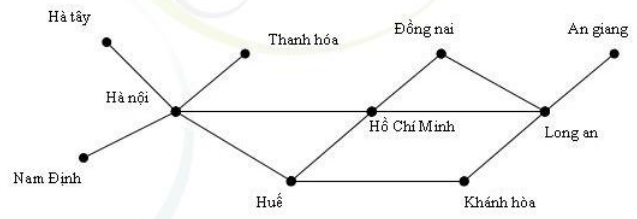
\includegraphics[scale=0.7]{./image/dothi_ex.png}
	\caption{Sơ đồ đường đi giữa các tỉnh}
	\end{center}
\end{figure}
\subparagraph{Đồ thị chính quy(Regular Graph)}(còn gọi là đồ thị đều) là một đồ thị trong đó mỗi đỉnh có số láng giềng bằng nhau, nghĩa là các đỉnh có bậc bằng nhau. Một đồ thị chính quy với các đỉnh có bậc bằng k được gọi là đồ thị chính quy bậc k.
\begin{itemize}
	\item Các đồ thị chính quy có bậc không lớn hơn 2 rất dễ nhận: đồ thị chính quy bậc 0 bao gồm các đỉnh cô lập, đồ thị chính quy bậc 1 bao gồm các cạnh không nối với nhau, và đồ thị chính quy bậc 2 bao gồm các chu trình không nối với nhau.
	\item Đồ thị chính quy bậc 3 còn được gọi là đồ thị bậc ba (cubic graph).
	\item Đồ thị chính quy mạnh là đồ thị chính quy mà mọi cặp đỉnh kề nhau đều có số láng giềng chung bằng nhau và mọi cặp đỉnh không kề đều có số láng giềng chung bằng nhau. Các đồ thị nhỏ nhất là đồ thị chính quy nhưng không chính quy mạnh là các đồ thị vòng (cycle graph) và đồ thị tròn (circulant graph) 6 đỉnh.
	\item Đồ thị đầy đủ $ K_{m}$ là đồ thị chính quy mạnh với mọi $ m$.
\end{itemize}
\begin{figure}[H]
	\begin{center}
	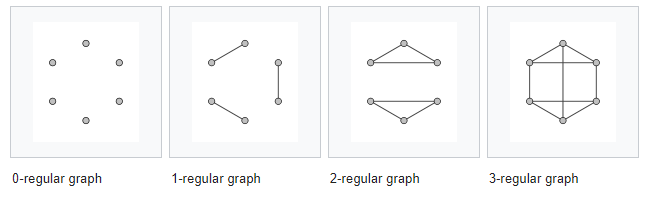
\includegraphics[scale=0.7]{./image/regular_graph.png}
	\caption{Đồ thị chính quy}
	\end{center}
\end{figure}

\paragraph{Một số tính chất cần chú ý:}
\begin{itemize}
	\item Một đồ thị chính quy vô hướng n đỉnh bậc k sẽ có $\frac{n \times k}{2}$ cạnh tương ứng.
	\item Một đồ thị vô hướng có n đỉnh và m cạnh $\rightarrow$ $ n >= k+1$.
	\item Đồ thị chính quy vô hướng sẽ có $n \times k $ là số chẵn.
\end{itemize}

\section{Giải quyết vấn đề}
\subsection{Xác định hướng đi}
Để giải quyết bài toán ta có 2 việc cần làm:
\begin{itemize}
	\item Xắp được đồ thị n đỉnh k trận không quan tâm đến việc nó đã là tối ưu hay chưa. Có nghĩa là ta đã xếp lịch được cho n vận động viên mà mỗi vận động viên đấu k trận.
	\item Tối ưu trạng thái hiện tại để thu được kết quả của bài toán theo ưu cầu là tổng điểm trung bình đối thủ của mỗi vận động viên không quá chênh lệch.
\end{itemize}

\subsection{Định nghĩa bài toán}
\subsubsection{Không gian bài toán}
Theo như lý thuyết đồ thị đã được nêu ở trên, ta có thể rút ra được không phải giá trị nào của n và k ta cũng có thể sắp xếp lịch cho vận động viên được. Ta sẽ có những ràng buộc được liệt kê sau:
\begin{enumerate}
	\item Số vận động viên phải lớn hơn số trận đấu mà họ sẽ đấu : $n >= k+1 $.
	\item Số trận đấu không được bé hơn 0 : $k > 0$.
	\item Số vận động viên không thể bé hơn hoặc bằng 1 : $n > 1$.
	\item Các vận động viên phải đấu đủ số trận là k : $\forall i,j \in n : k_i = k_j$
	\item Đồ thị cần xếp có $\frac{n \times k}{2} $ trận : $n \times k$ là số chẵn.
\end{enumerate}
\newpage

\subsubsection{Phân rã bài toán thành bài toán nhỏ hơn}
Bài toán xếp lịch thi đấu cho n vận động viên với k trận đấu sẽ được chia thành bài toán nhỏ hơn được gọi như các quy luật:
\begin{enumerate}
	\item Với $k = 1$: $(n, 1)$. Ta sẽ bắt cặp bất kì trọng n vận động viên. Mỗi cặp sẽ gồm 2 vận động viên đấu với nhau.
	\item[] Vd : $(4, 1)= (1,2,3,4) = \lbrace [1, 2], [3, 4] \rbrace$Với 1,2,3,.. đại điện cho id của từng vận động viên. [1,2].. đại diện từng trận của vận động viên.	
	\begin{figure}[H]
	 	\centering
	 	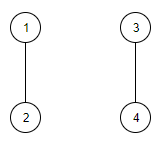
\includegraphics[scale=0.7]{./image/k1.png}
	 	\caption{Xếp trận đấu cho n = 4 và k = 1.}
	 \end{figure}
	 
	\item Với $k = 2$: $(n, 2)$. Ta sẽ xếp trận dựa trên quy luật chuyển đồ thị thành hình tròn như hình sau. Lúc này mỗi vận động viên đã có đủ k trận thỏa mãn theo yêu cầu bài toán.
	 \begin{figure}[H]
	 	\centering
	 	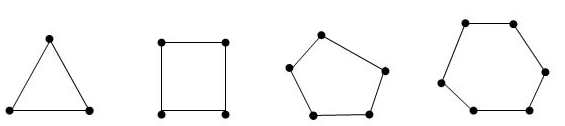
\includegraphics[scale=0.7]{./image/dothivong.png}
	 	\caption{Xếp trận đấu cho k = 2}
	 \end{figure}
	 
	 \item Với $k = \frac{n}{2}$: $(n, \frac{n}{2})$ Ta sẽ chia làm 2 nhóm để xếp lịch mỗi nhóm chứa $\frac{n}{2}$ vận động viên. Khi đó ta sẽ xếp lịch theo quy luật mỗi thành viên nhóm này sẽ đấu với toàn bộ thành viên nhóm còn lại.
	 \item[] Vd: $(6,3) = (1,2,3,4,5,6) = \lbrace \theta \rbrace $
	 \begin{figure}[H]
	 	\centering
	 	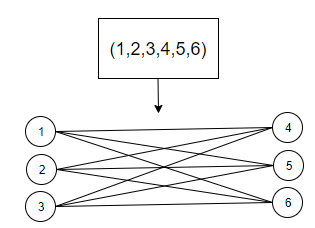
\includegraphics[scale=0.7]{./image/kn_2.png}
	 	\caption{Xếp trận đấu cho $k = \frac{n}{2}$}
	 \end{figure}
	 \newpage
	 
	 
	 \item Với k = n - 1: (n, n-1) Ta sẽ cho 1 thằng đấu với tất cả các thằng còn lại đối với mọi vận động viên.
	 \item[] Vd $(7,6) = (1,2,3,4,5,6,7) = \lbrace \theta \rbrace $
	 \begin{figure}[H]
	 	\centering
	 	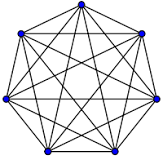
\includegraphics[scale=0.7]{./image/k_n_1.png}
	 	\caption{Xếp trận đấu cho $n = 7$ và $k = 6$}
	 \end{figure}
	 
	 \item Với $k > \frac{n}{2}$: (n,k) Ta sẽ chia 2 nhóm:
	 \begin{enumerate}
	 	\item Nhóm 1: có k vận động viên.
	 	\item Nhóm 2: có n - k vận động viên.
	 \end{enumerate}
	 \item[] Ta tiến hành cho từng thành viên nhóm 2 sẽ đấu với toàn bộ thành viên nhóm 1. Khi đó nhóm 2 đã đấu đủ số trận đấu cần thiết của nó.
	 \item[] Lúc này nhóm 1 đã đấu được n - k trận. Điều đó có nghĩa nó sẽ phải đấu thêm $k - (n-k) = 2k - n$ trận nữa thì mới đủ k trận.
	 \item[] Vì nhóm 1 đấu chưa đủ trận nên ta sẽ cho từng thành viên trong nhóm 1 đấu với nhau $2k - n$ trận. Quy bài toán về xếp lịch thi đấu cho $(n-k, 2k - n)$.
	 \item[] Ví dụ Xếp lịch cho trường hợp (7,4) Chia làm 2 nhóm 1 nhóm có 4 vđv , 1 nhóm có 3 vđv. Sau khi xếp trận cho nhóm có 3 vđv thì nhóm có 4vđv vẫn còn thiếu 1 trận nên ta sẽ sắp lịch cho nhóm còn lại $\rightarrow (4, 1)$
	 \begin{figure}[H]
	 	\centering
	 	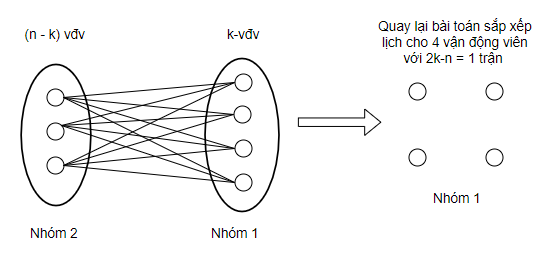
\includegraphics[scale=0.7]{./image/ex1_large.png}
	 	\caption{Xếp trận đấu cho $n = 7$ và $k = 4$}
	 \end{figure}
	 
	 \newpage
	 \item Với $k < \frac{n}{2}$ và n là số chẵn. Ta sẽ chia thành 2 nhóm:
	 \begin{enumerate}
	 	\item Nhóm 1: có k + 1 vận động viên.
	 	\item Nhóm 2: có n - (k + 1) vận động viên.
	 \end{enumerate}
	 \item[] Vì $k < \frac{n}{2}$ nên nhóm 2 sẽ có tổng số vđv lớn hơn $k + 1$. Lúc này ta tiến hành quy về bài toán nhỏ hơn là sắp xếp lịch lại cho từng nhóm: nhóm 1 (k+1,k) -- nhóm 2 (n-k-1, k).
	 \item[] Xét nhóm 1 ta dễ dàng thấy được đây là bài toán xếp lịch cho trường hợp (n, n-1) đã được nêu ở trên. Tương tự xử lý cho nhóm 2.
	 \item[] Sau đây là 1 ví dụ đại diện cho trường hợp này: $(10, 4)$
	 \begin{figure}[H]
	 	\centering
	 	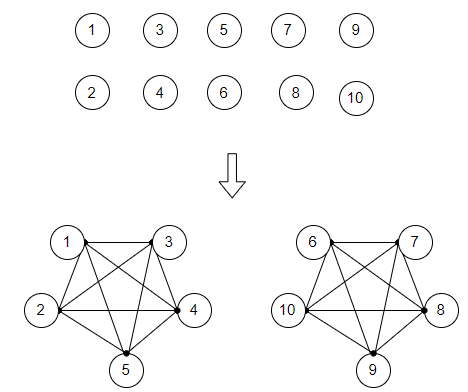
\includegraphics[scale=0.7]{./image/ex1_nho.png}
	 	\caption{Xếp trận đấu cho $n = 10$ và $k = 4$}
	 \end{figure}
	 \item[]Một ví dụ khác cho trường hợp này: $(12, 4)$
	 \begin{figure}[H]
	 	\centering
	 	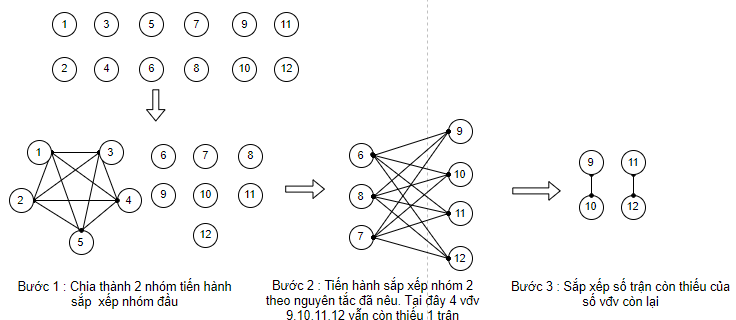
\includegraphics[scale=0.7]{./image/ex2_nho.png}
	 	\caption{Xếp trận đấu cho $n = 12$ và $k = 4$}
	 \end{figure}
	 
	 \newpage
	 \item Với $k < \frac{n}{2}$ và n là số lẻ. Vì n là số lẻ nên ta có thể lấy 1 vđv ra xếp riêng số vđv còn lại ta có thể phân làm 2 nhóm có số vđv bằng nhau. Như vậy ta có 3 nhóm : 
	 \begin{enumerate}
	 	\item Nhóm 1: Gồm 1 vđv.
	 	\item Nhóm 2: Gồm $\frac{n-1}{2} $ vđv.
	 	\item Nhóm 3: Gồm $\frac{n-1}{2} $ vđv.
	 \end{enumerate}
	 \item[] Ta sẽ sắp xếp trận như hình minh họa sau đây cho ví dụ sắp xếp trường hợp (9,4):
	 \begin{figure}[H]
	 	\centering
	 	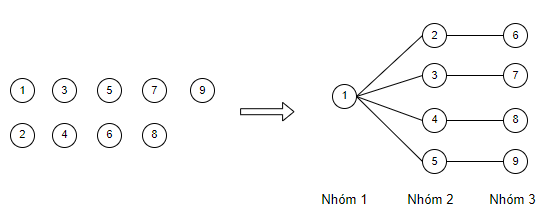
\includegraphics[scale=0.7]{./image/kle.png}
	 	\caption{Xếp trận đấu cho $n = 9$ và $k = 4$}
	 \end{figure}
	 \item[] Quy luật sắp xếp theo hình trên được mô tả lại như sau: Ghép trận vđv nhóm 1 với tất cả vđv thuộc nhóm 2, mỗi vđv thuộc nhóm 2 ta sẽ ghép với 1 vđv ở nhóm 3.
	 \item[] Như thế ta có được nhóm 1 đã đủ số trận đấu, nhóm 2 mỗi vđv đã đấu 2 trận là 1 trận với nhóm 1 và 1 trận với nhóm 3, nhóm 3 mỗi vđv đã đấu được 1 trận khi được sắp với nhóm 2.
	 \item[] Ta có thể rút ra được nhóm 2 sẽ còn thiếu k - 2 trận và nhóm 3 sẽ có thiếu k - 1 trận đối với mỗi vđv.
	 \item[] Lý do chia như vậy vì khi chia nhóm 2 và 3 mỗi nhóm đều có $\frac{n-1}{2}$ vđv và ta có $k < \frac{n}{2}$ Nên chắc chắn số phần tử trong nhóm 2 và 3 luôn nhỏ hơn k. Từ đó ta đã có thể quy về bài toán ban đầu là sắp xếp lịch cho nhóm 2 là $(\frac{n-1}{2} , k - 2)$ và sắp xếp lịch cho nhóm 3 là $(\frac{n-1}{2} , k - 1)$ 
	 
\end{enumerate}
\subsection{Tối ưu trạng thái mục tiêu}
Theo như phương pháp xây dựng trạng thái (khởi tạo đồ thị) như đã trình bày ở trên. Em quyết định chọn cách tối ưu từng bài toán con cho từng trường hợp của k như đã liệt kê.\\
Theo như cách sắp xếp chủ yếu là phân n vđv thành từng nhóm nhỏ khác nhau nên để trạng thái mục tiêu là tốt nhất thì việc lựa chọn thí sinh nào vào nhóm nào mới hợp lý. Như thế thuật toán này sẽ tối ưu trong việc \textbf{chọn lựa} để phân nhóm. Thuật toán này mô phỏng gần giống với giải thuật leo đồi (Hill Climbing) nhưng nó được xử lý tại lúc sinh ra trạng thái tập hợp các thí sinh để phân nhóm tại thời điểm đang xét k trong những trường hợp nêu ở mục trên chứ không phải toàn bộ bài toán ban đầu.\\
$\ast$\textbf{\textit{Chú ý}} : Nhiệm vụ đầu tiên của thuật toán là sắp xếp lại điểm của các vđv theo thứ tự điểmcủa họ từ nhỏ để lớn. Gán id cho chúng theo thứ tự 1,2,... n.
\subsubsection{Định nghĩa trạng thái}
\paragraph{Trạng thái}: chứa từ $1 \rightarrow 3$ danh sách tùy thuộc vào trường hợp k. Mỗi danh sách chứa $n_i$ phần tử, mỗi phần tử trong danh sách này này đại diện cho 1 vđv.\\
$(n,k) = ( 1, 2, 3,..n )$. Với 1,2,3,.. đại điện cho id của từng vận động viên.\\
Ví dụ: $(3, 1)= ( 1,2,3 )$.Trường hợp này k = 1 ta chỉ sinh 1 danh sách chưa 3 vđv.
\paragraph{Trạng thái khởi đầu}: $(n,k)= ( 1,2,..n )$

\paragraph{Trạng thái mục tiêu}: $(n,k)= ( a,b,..n )$. Với a,b,.. là những vđv thích hợp nhất trong danh sách để tiến hành sắp xếp trận theo quy luật. 
\subsubsection{Luật di chuyển trạng thái}
Ta có luật di chuyển cho trạng thái sẽ tùy thuộc vào giá trị k chúng ta đang xét. Sau đây là phân tích về việc tối ưu và cách thức chuyển trạng thái. Để dễ hiểu và như thuật toán quy định như trên các vđv đã được sắp xếp theo thứ tự điểm từ nhỏ đến lớn nên các ví dụ trình bày sau sẽ coi như id là điểm của mỗi vđv. \\
$\ast$\textbf{\textit{Giải thích}} : vdv[1] sẽ có điểm thấp hơn vđv[2] vì danh sách này đã được sắp xếp. Khi sắp lịch xong thuật toán này sẽ duyệt lại danh sách theo thứ tự ban đầu để xuất ra kết quả. Ta sẽ coi như vđv[1] sẽ có điểm là 1, vđv[2] sẽ có điểm là 2,.. Quy ước như vậy sẽ không ảnh hưởng đến việc điểm của 2 vđv thực tế chênh lệch nhau trong trường hợp xấu nhất bởi vì điểm của chúng đã thực sự thấp hơn tại một khoảng nào đó nên việc quy định như vậy sẽ không ảnh hưởng đến kết quả bài toán.
\begin{enumerate}
	\item \textbf{Với} $k = 1$: Trường hợp này không cần phải tìm ra danh sách chia tốt nhất vì dù có chia như thế nào thì luôn sẽ có vđv phải đấu với vđv có điểm thấp nhất, tương tự như trường hợp điểm cao nhất.
	\item[] Không cần tối ưu.
	
	\item \textbf{Với $k = 2$:}  Ta sẽ xét ví dụ trường hợp n = 5
	\item[] Trạng thái khởi đầu : [1,2,3,4,5]. Dựa trên trạng thái này nếu xếp lịch theo quy luật ta sẽ nối 1 với 2, 2 với 3,.. 5 với 1. Như vậy ta được một đồ thị là vòng tròn. Từ đó ta có thể suy ra bảng điểm của mỗi vđv như sau:
	\begin{figure}[H]
		\centering
		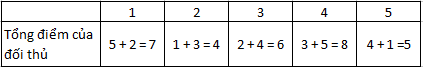
\includegraphics[scale=1]{./image/hinh1.png}
	\end{figure}	 
	\item[] Từ bảng trên ta có thể thấy được giá trị min, max của tổng điểm rơi vào vđv 2 và 4. Ta sẽ tối ưu hóa giá trị |max - min| này càng tiến về 0 thì giá trị ta thu được càng là tốt.
	\item[] Bởi vì điểm 5 là max trong 5 vđv nên nó sẽ đóng góp vào giá trị max của tổng điểm và điểm 1 là min nên nó sẽ ảnh hưởng vào giá trị của tổng điểm. Nên để max của tổng điểm giảm dần ta sẽ swap vị trí của điểm 5 với điểm gần nó, tưởng tự với điểm min của tổng điểm tăng dần ta sẽ swap điểm thấp nhất và điểm thấp nhì gần nó. Ta sẽ swap vị trí của 2 cặp  tiếp theo không tính những cặp đã swap rồi cho đến khi gặp phần tử trung tâm.
	\item[] Ta sẽ có kết quả cuối cùng: [2,1,3,5,4] sẽ cho ra bảng kết quả tốt hơn trạng thái ban đầu có được. Khi đây chêch lệnh max min của tổng điểm là |7 - 5| = 2:
	\begin{figure}[H]
		\centering
		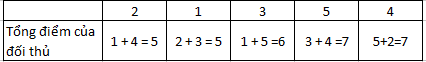
\includegraphics[scale=1]{./image/hinh2.png}
	\end{figure}	
	\item[] Tương tự cho ví dụ n = 8. Ta sẽ có trạng thái khởi đầu là:
	\item[][1,2,3,4,5,6,7,8] $\rightarrow$ [2,1,3,4,5,6,8,7] $\rightarrow$ [2,1,4,3,6,5,8,7]
	
	\item \textbf{Với} $k = \frac{n}{2}$: Ta sẽ có trạng thái khởi đầu gồm 2 danh sách. Một danh sách chứa 1 nửa vđv, 1 danh sách chứa các vđv còn lại.
	\item[] Ví dụ minh họa: n=8 k=4 $\rightarrow$ Trạng thái khởi đầu [1,2,3,4] và [5,6,7,8]. Bởi vì 1 vđv thuộc 1 trọng 2 danh sách sẽ đấu với toàn bộ danh sách còn lại. Ta sẽ tối ưu làm thế nào để đưa tổng điểm của 2 danh sách là sấp xĩ nhau
	\item[] Ta có chênh lệch giữa $sum[list score 1]$ và $ sum[list score 2]$ là alpha. Để tìm được trường hợp tốt nhất thì alpha $\simeq $ 0.
	\item[] Hàm lượng giá: $sum[list score 1] \simeq sum[list score 2]$
	\item[] Tại vì ban đầu ta đã sắp xếp vị trí từ nhỏ để lớn nên list 1 luôn sẽ có điểm nhỏ hơn hoặc bằng list 2. Do đó điều kiện thực hiện tối ưu là $sum[list score 1] < sum[list score 2]$. Ta sẽ swap các phần tử sao cho thỏa mãn điều kiện tối ưu.
	\item[] Theo như code hiện thực trạng thái mục tiêu của trường hợp trên như sau : [8,2,3,4] và [5,6,7,1] alpha = |sum(list2) - sum(list1)| = 3 đây là con số nhỏ nhất có thể tìm được nên ta coi nó là trường hợp tốt nhất. Công việc còn lại là ta sắp trận đánh của 2 list theo quy luật ta sẽ được kết quả tốt nhất có thể tìm thấy.
	
	\item \textbf{Với} $k =n-1 $:Trường hợp này không cần phải tìm ra danh sách chia tốt nhất vì 1 vđv bất kì sẽ luôn đấu với số vđv còn lại.
	\item[] Không cần tối ưu.
	
	\newpage
	\item \textbf{Với} $k > \frac{n}{2}$ Ta sẽ có trạng thái khởi đầu gồm 2 danh sách: danh sách 1 chưa k vđv, danh sách 2 chứa n-k vđv.
	\begin{figure}[H]
		\centering
		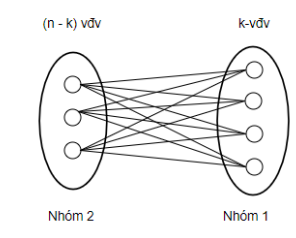
\includegraphics[scale=0.7]{./image/hinh3.png}
	\end{figure}
	\item[] Từ hình trên ta có thể thấy được tổng điểm của mỗi đối thủ thuộc danh sách 1 sẽ là tổng số điểm của danh sách 2 = $sum(list1)$. 
	
	\item[*] $max(min)\_k\_ptu(listX)$ : là tổng điểm của k phần tử có điểm cao nhất(thấp nhất) trong list X
	\item[] Tổng điểm của mỗi phần tử trong danh sách 2 sẽ chạy từ:
	\begin{center}
	\item[] $sum(list2) + min\_k\_ptu(list1) \leq X \leq sum(list2) + max\_k\_ptu(list1)$.
	\end{center}
	\item[] Hàm lượng giá trong trường hợp này sẽ là:
	\begin{center}
	 $sum(list1) \simeq  sum(list2) + max\_k\_ptu(list1)$
	\end{center}
	\item[] Ta sẽ swap các phần tử giữa 2 list sao cho giá trị độ chênh lệch của hàm lượng giá là nhỏ nhất. Bởi vì khi thu hẹp dần khoảng cách của 2 giá trị max này ta sẽ thu được danh sách có độ chênh lệch tổng điểm trung bình là gần bằng nhau.
	
	\item \textbf{Với} $k < \frac{n}{2}$ Cho cả trường hợp n chẵn và n lẻ. Hàm lượng giá của 2 trường hợp này cũng giống như hàm lượng giá ở trường hợp $k > \frac{n}{2}$. Bước chuyển trạng thái cũng chính là cách swap 2 phần tử ở các danh sách với nhau cho đến khi hàm lượng giá thỏa mãn. Thu được kết quả là các danh sách ta chỉ còn 1 công việc là sắp xếp theo quy luật đã đề ra.
\end{enumerate}

\section{Kết quả đạt được}
\subsection{Sắp lịch cho trường hợp n = 8, k = 4}
	\begin{figure}[H]
		\centering
		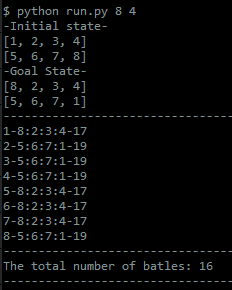
\includegraphics[scale=0.7]{./image/kq1.png}
	\end{figure}
	 Phần trên cùng là trạng thái khởi đầu. Kế tiếp là trạng thái mục tiêu. Mục kế tiếp thể hiện danh sách vđv từ 1..n phần giữa là id của những đối thủ nó sẽ đấu, cuối cùng là tổng điểm của các đổi thủ của nó.
	
\subsection{Sắp lịch cho trường hợp n = 18, k = 11}
	\begin{figure}[H]
		\centering
		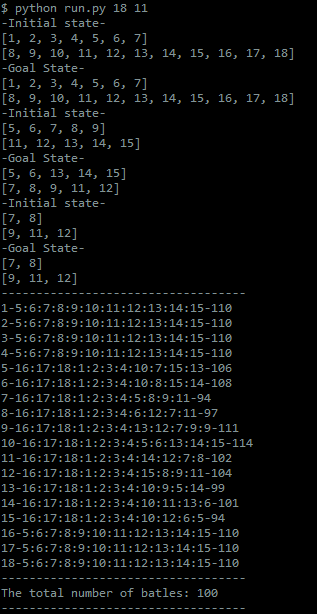
\includegraphics[scale=0.5]{./image/kq2.png}
	\end{figure}
	Việc xuất hiện nhiều trạng thái khởi đầu như vậy là do giải thuật này giảm kích thước của bài toán lớn thành các bài toán con nhỏ để giải quyết. Mỗi lần hoàn thành 1 bài toán con sẽ có 1 trạng thái khởi đầu và mục tiêu khác nhau do đó sẽ tối ưu được bài toán lớn.
	
\section{Quá trình kiểm tra và đánh giá}
	\subsection{Tạo testcase để kiểm tra}
	Để tiện cho việc kiểm tra trên nhiều testcase khác nhau, em có điều chỉnh code thêm tùy chọn số n và k. Do vậy chúng ta có 2 cách để chạy code chương trình:
	\begin{center}
		\textbf{python 1613989.py n k }\\
		hoặc\\[0.2cm]
		\textbf{python 1613989.py}\\
		
	\end{center}		
	Đối với cách này theo ưu cầu của đề chương trình sẽ đọc dữ liệu từ file "input.txt".\\
	Trong code sẽ tự động sinh ra danh sách n vđv mỗi vđv có 1 giá trị random điểm ngẫu nhiên. Sẽ giúp việc tạo test case dễ hơn. 
	\paragraph{Cách sinh test}: Ta sẽ sinh điểm của từng thí sinh ngẫu nhiên theo code sau: a là cận dưới, b là cận trên, x là thứ tự id của từng vđv.
	\begin{lstlisting}
		for x in range(1,n+1):
            _a = random.randint(1,90)
            _b = random.randint(_a,90)
            a = int(random.randint(_a,_b))
            ls.append(Candidate(x,a))
	\end{lstlisting}
	
	\subsection{Đánh giá giải thuật}
	\paragraph{Vấn đề về đệ quy} Giải thuật có sử dụng kĩ thuật đệ quy nên khi xử lý bài toán quá lớn sẽ dễ gây break chương trình.
	\paragraph{Vấn đề có thể xảy ra nhưng không được giải quyết:} Trong một vài trường hợp việc tối ưu bài toán nhỏ có thể đạt tối ưu tốt nhưng khi gộp lại bài toán lớn thì bài toán lớn có thể sẽ không được tối ưu.
	\paragraph{Vấn đề tối ưu nhất} Chưa có cách kiểm tra toàn bộ trường hợp liệu rằng nó đã là tốt nhất hay chưa. Thuật toán chỉ tìm được trạng thái tốt nhất có thể nên trong một vài trường hợp, giải pháp này sẽ bị rơi vào tối ưu cục bộ.
	
	\subsection{Số lượng file đính kèm}
	Bài nộp online bao gồm 2 file : \textbf{1613989.pdf} và \textbf{1613989.py}.
\newpage
\begin{thebibliography}{80}
	\bibitem{latexcompanion} Tri tue nhan tao = Thong minh + Giai thuat (2008)- Cao Hoang Tru
	\bibitem{latexcompanion} Artificial Intelligence: A Modern Approach (2009)- Stuart Russell and Peter Norvig
	\bibitem{latexcompanion} \url{https://en.wikipedia.org/wiki/Regular_graph}
	\bibitem{latexcompanion} Slide: Artificial Intelligence(Bkel)
\end{thebibliography}

\end{document}
